\documentclass[conference]{IEEEtran}
\IEEEoverridecommandlockouts
% The preceding line is only needed to identify funding in the first footnote. If that is unneeded, please comment it out.
\usepackage{cite}
\usepackage{amsmath,amssymb,amsfonts}
\usepackage{algorithmic}
\usepackage{graphicx}
\usepackage{textcomp}
\usepackage{xcolor}
\usepackage{tabularx}
\usepackage{multirow}
\usepackage{graphics} % for pdf, bitmapped graphics files
\usepackage{subfig}
\usepackage{subcaption}
\usepackage{hyperref}
\usepackage{academicons}
\usepackage{xcolor}
\usepackage{listings}
\usepackage{tabularx} % Asegúrate de incluir este paquete

\usepackage{tikz}
\usetikzlibrary{shapes.geometric, arrows}

\usetikzlibrary{shapes.geometric, arrows}

\tikzstyle{startstop} = [rectangle, rounded corners, minimum width=3cm, minimum height=1cm,text centered, draw=black, fill=red!30]
\tikzstyle{process} = [rectangle, minimum width=3cm, minimum height=1cm, text centered, draw=black, fill=blue!30]
\tikzstyle{arrow} = [thick,->,>=stealth]


\def\BibTeX{{\rm B\kern-.05em{\sc i\kern-.025em b}\kern-.08em
		T\kern-.1667em\lower.7ex\hbox{E}\kern-.125emX}}

% Color Enlace
\definecolor{colorEnlace}{RGB}{0, 0, 0}
\hypersetup{
	colorlinks=true,
	linkcolor=colorEnlace,
	citecolor=colorEnlace,
	urlcolor=colorEnlace,
	pdfauthor={Davis Bremdow Salazar Roa},
	pdftitle={Sistemas Embebidos}
}
\definecolor{mybg}{rgb}{0.97,0.97,0.97}
\definecolor{mygray}{gray}{0.4}
\definecolor{mygreen}{rgb}{0,0.6,0}
\definecolor{myblue}{rgb}{0,0,0.8}
\definecolor{mypurple}{rgb}{0.58,0,0.82}
\definecolor{myred}{rgb}{0.7,0,0}

\lstdefinelanguage{MatlabEnhanced}{
	language=Matlab,
	morekeywords={[2]linspace,plot,title,xlabel,ylabel,legend,grid},
	morekeywords={[3]sin,cos,exp,log,sqrt},
	keywordstyle=\color{myblue}\bfseries,
	keywordstyle=[2]\color{mypurple},
	keywordstyle=[3]\color{myred},
	commentstyle=\color{mygreen}\itshape,
	stringstyle=\color{mygray},
	morecomment=[l]%
}

\lstset{
	language=MatlabEnhanced,
	backgroundcolor=\color{mybg},
	frame=single,
	basicstyle=\ttfamily\small,
	showstringspaces=false,
	numbers=none,              %
	xleftmargin=0pt,           %
	framexleftmargin=0pt,      
	framexrightmargin=0pt,
	framextopmargin=2pt,
	framexbottommargin=2pt,
	breaklines=true,
	tabsize=1,
}

% Control 
\usepackage{amsmath}
\begin{document}
	
	\title{Modulación FM - Análisis de una señal de voz}
	\author{
		\makebox[\textwidth][c]{\large\textbf{Universidad Nacional de San Antonio Abad del Cusco}}\\
		\makebox[\textwidth][c]{\normalsize\textit{Escuela profesional de Ingeniería Electrónica}}\\
		\makebox[\textwidth][c]{\normalsize\textit{Laboratorio de Circuitos Electrónicos III}}\\
		\and
		\IEEEauthorblockN{Ing. Milton Velasquez Curo}
		\IEEEauthorblockA{Ingeniero Electrónico \\
			Cusco, Perú \\
			milton.velasquez@unsaac.edu.pe}
		\and
		\IEEEauthorblockN{Ruth Juana Espino Puma - 185746}
		\IEEEauthorblockA{Estudiante de Ingeniería Electrónica \\
			Cusco, Perú \\
			184657@unsaac.edu.pe}
		\and
		\IEEEauthorblockN{Davis Bremdow Salazar Roa - 200353}
		\IEEEauthorblockA{Estudiante de Ingeniería Electrónica \\
			Cusco, Perú \\
			200353@unsaac.edu.pe}
	}
	
	\maketitle
	\begin{abstract}
		La modulación es un proceso fundamental en las telecomunicaciones que consiste en variar una o más propiedades de una señal portadora (como amplitud, frecuencia o fase) en función de una señal de información o mensaje. Este proceso permite transmitir información a largas distancias de manera eficiente, minimizando interferencias y aprovechando mejor el espectro de frecuencias. Existen varios tipos de modulación, entre ellos la modulación en amplitud (AM), frecuencia (FM) y fase (PM), cada una con características y usos específicos según las necesidades del sistema de comunicación.
		
	\end{abstract}
	
	\begin{IEEEkeywords}
		Modulación, portadora, señal, índice de modulación, amplitud, frecuencia, fase, transmisión, espectro, distorsión.
	\end{IEEEkeywords}
	
	%% Contenido del documento
	
	\section{ Modulación FM }
	Para realizar la modulación FM de una señal de voz existen varios caminos a tomar dentro de MATLAB dentro de los cuales se pueden apreciar la función fmmod o el uso de las herramientas integrales para definir la expresión FM resultante.
	
	Para este propósito se hizo uso del código mostrado en el listing \ref{lst:modulacion-fm} define una modulación mediante el empleo de la función $cumsum()$ la cual se encarga de integrar la señal moduladora.
	
	\begin{lstlisting}[numbers=none, caption="", label=lst:modulacion-fm]
		%% Parámetros de la senal de informacion
		fm = 15;
		a = 2;
		
		%%  Parametro de la portadora
		fc = 100;
		A = 5;
		
		Ts = 1/(1000*fc);
		Fs = 1/Ts;
		t = 0: Ts : 0.5 - Ts;
		
		ft = a*sin(2*pi*fm*t);
		
		%% Modulación AM
		fi = A*cos(2*pi*fc*t + 2*pi*cumsum(ft)*Ts);
	\end{lstlisting}
	
	El agregado para este procedimiento se realiza mediante la definición de una variable que se encarga de recuperar la información de un archivo .wav en la cual se tiene registrado un audio de 2 segundos, en el listing \ref{lst:audio-matlab} se define estas líneas de código.
	
	\begin{lstlisting}[caption={Recuperación del archivo del audio}, numbers=none, label=lst:audio-matlab]
		y = audioread("audio.wav");
	\end{lstlisting}
	
	En este pequeño fragmento de código y la variable $y$ almacenan 16000 muestras registradas para 2 segundos de grabación.
	
	Ya con los datos del archivo de audio (señal moduladora), esta se puede emplear para realizar la modulación de la señal de información mediante la portadora, sin embargo antes de ello es necesario conocer las componentes de frecuencia de la señal de audio para hacer uso de una portadora adecuada con la cual se pueda adecuar la señal de información para su traslado en frecuencia.
	
	Una primera aproximación en frecuencia para la señal de audio se puede obtener mediante la transformada de Fourier la cual nos brindará que componentes (tonos u otros) se encuentran más representado en este dominio.
	
	\begin{figure}[h]
		\centering
		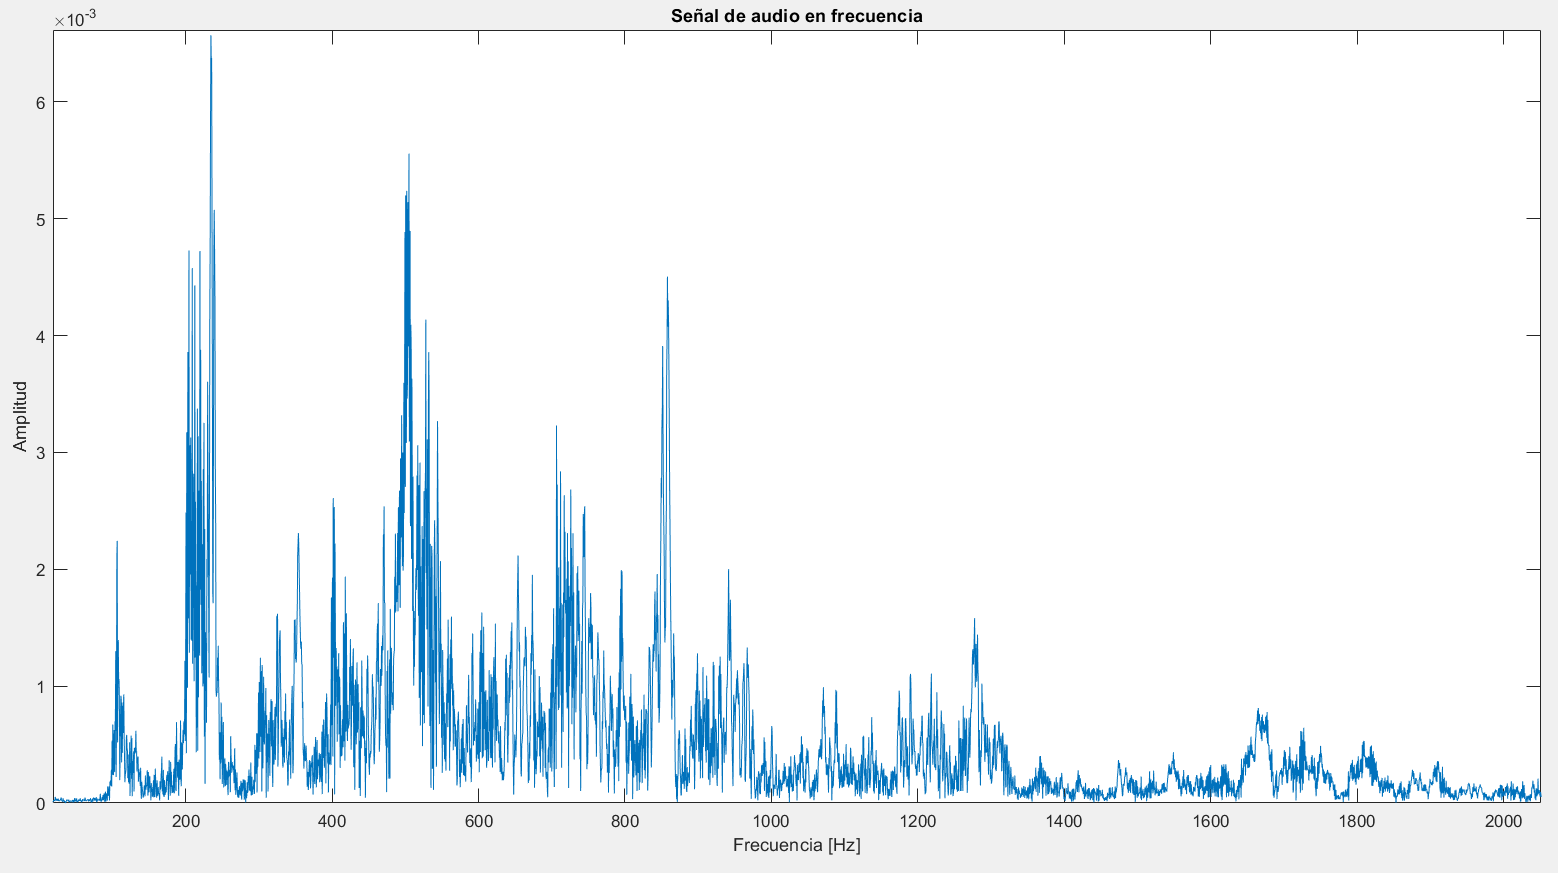
\includegraphics[width=0.5\textwidth]{media/fft-audio}
		\caption{Transformada de Fourier - Audio}
		\label{fig:fft-audio}
	\end{figure}
	
	
	En la figura \ref{fig:fft-audio} se puede apreciar el espectro de la señal de audio en la cual se puede apreciar 3 tonos significativos en:
	\begin{itemize}
		\item $f_1 = 235 [Hz] $
		\item $f_2 = 505 [Hz]$
		\item $f_3 = 858 [Hz]$
	\end{itemize}
	
	Siendo necesario el empleo de una portadora superior a la máxima frecuencia resultante para evitar comportamientos inesperados durante este proceso.
	
	\section{  }
	
	\bibliographystyle{IEEEtran}
	\bibliography{biblio}
\end{document}
